% compile with XeLaTeX
\documentclass[dvipsnames,mathserif, handout]{beamer}
%\setbeamerfont{title}{size=\tiny}
\setbeamertemplate{footline}[frame number]
\setbeamercolor{footline}{fg=black}
\setbeamerfont{footline}{series=\bfseries}

\usepackage{tikz, babel, ulem}
\usepackage[export]{adjustbox}

\usetheme{Frankfurt}%1
%\usetheme{Darmstadt}%1

\setbeamerfont*{itemize/enumerate body}{size=\fontsize{9}{11}}
\setbeamerfont*{itemize/enumerate subbody}{parent=itemize/enumerate body}
\setbeamerfont*{itemize/enumerate subsubbody}{parent=itemize/enumerate body}

\makeatother

%% for RTL liste
%\makeatletter
%\newcommand{\RTListe}{\raggedleft\rightskip\leftm}
%\newcommand{\leftm}{\@totalleftmargin}
%\makeatother
%
%% RTL frame title
%\setbeamertemplate{frametitle}
%{\vspace*{-1mm}
%  \nointerlineskip
%    \begin{beamercolorbox}[sep=0.3cm,ht=2.2em,wd=\paperwidth]{frametitle}
%        \vbox{}\vskip-2ex%
%        \strut\hskip1ex\insertframetitle\strut
%        \vskip-0.8ex%
%    \end{beamercolorbox}
%}
%% align subsection in toc
%\makeatletter
%\setbeamertemplate{subsection in toc}
%{\leavevmode\rightskip=5ex%
%  \llap{\raise0.1ex\beamer@usesphere{subsection number projected}{bigsphere}\kern1ex}%
%  \inserttocsubsection\par%
%}
%\makeatother
%
%% RTL triangle for itemize
%\setbeamertemplate{itemize item}{\scriptsize\raise1.25pt\hbox{\donotcoloroutermaths$\blacktriangleleft$}} 
%
%%\setbeamertemplate{itemize item}{\rule{4pt}{4pt}}
%
%\defbeamertemplate{enumerate item}{square2}
%{\LR{
%    %
%    \hbox{%
%    \usebeamerfont*{item projected}%
%    \usebeamercolor[bg]{item projected}%
%    \vrule width2.25ex height1.85ex depth.4ex%
%    \hskip-2.25ex%
%    \hbox to2.25ex{%
%      \hfil%
%      {\color{fg}\insertenumlabel}%
%      \hfil}%
%  }%
%}}
%
%\setbeamertemplate{enumerate item}[square2]

%\setbeamertemplate{footline}{} %gets rid of footer completely
\setbeamertemplate{navigation symbols}{}


\titlegraphic { 
\begin{tikzpicture}[overlay,remember picture, opacity=0.1,]
\node[] at (0, 2.9){
    
\includegraphics[width=0.63\textwidth]{iCapital_logo_RGB.png}
};\end{tikzpicture}}

%\setbeamertemplate{caption}[numbered]
\setbeamertemplate{caption}{\raggedright\insertcaption\par}

\begin{document}

\rightskip\rightmargin
\title{Asset Level CMAs}
\author{ \Large \textbf{} }
\institute{\large\textbf{}\\
Arnav Sheth \\
iCapital Network}
\footnotesize{\date{February 29, 2024 }


\begin{frame}
	\maketitle
\end{frame}

\begin{frame}{Summary}
	\footnotesize \tableofcontents
\end{frame}

\section{Basic Plan}

\begin{frame}{Methodology}
	Haddad et al, Review of Financial Studies 33(2020): pp.1980-2018 
	\begin{figure}[!ht]
		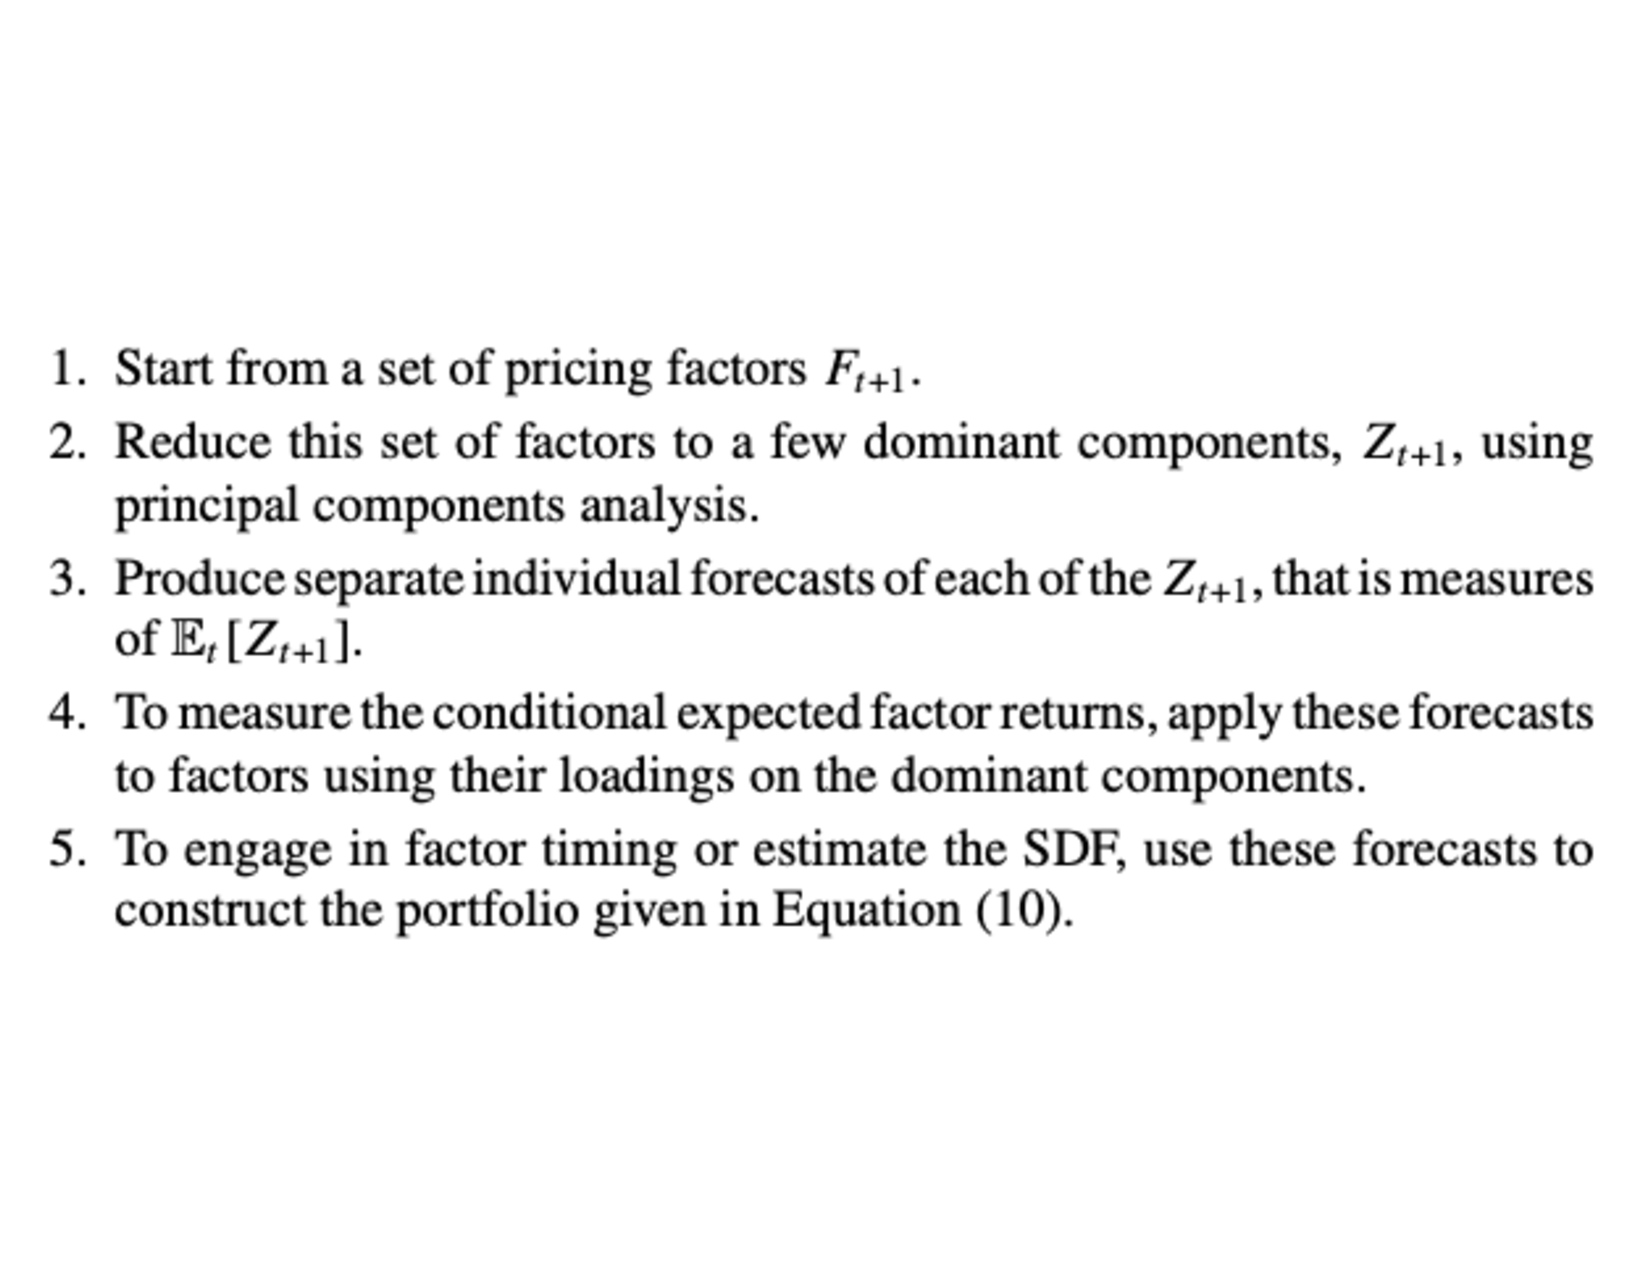
\includegraphics[width=300pt]{Steps_orig.pdf}
	\end{figure}
\end{frame}

\begin{frame}{Methodology}
	Haddad et al, Review of Financial Studies 33(2020): pp.1980-2018 
	\begin{figure}[!ht]
		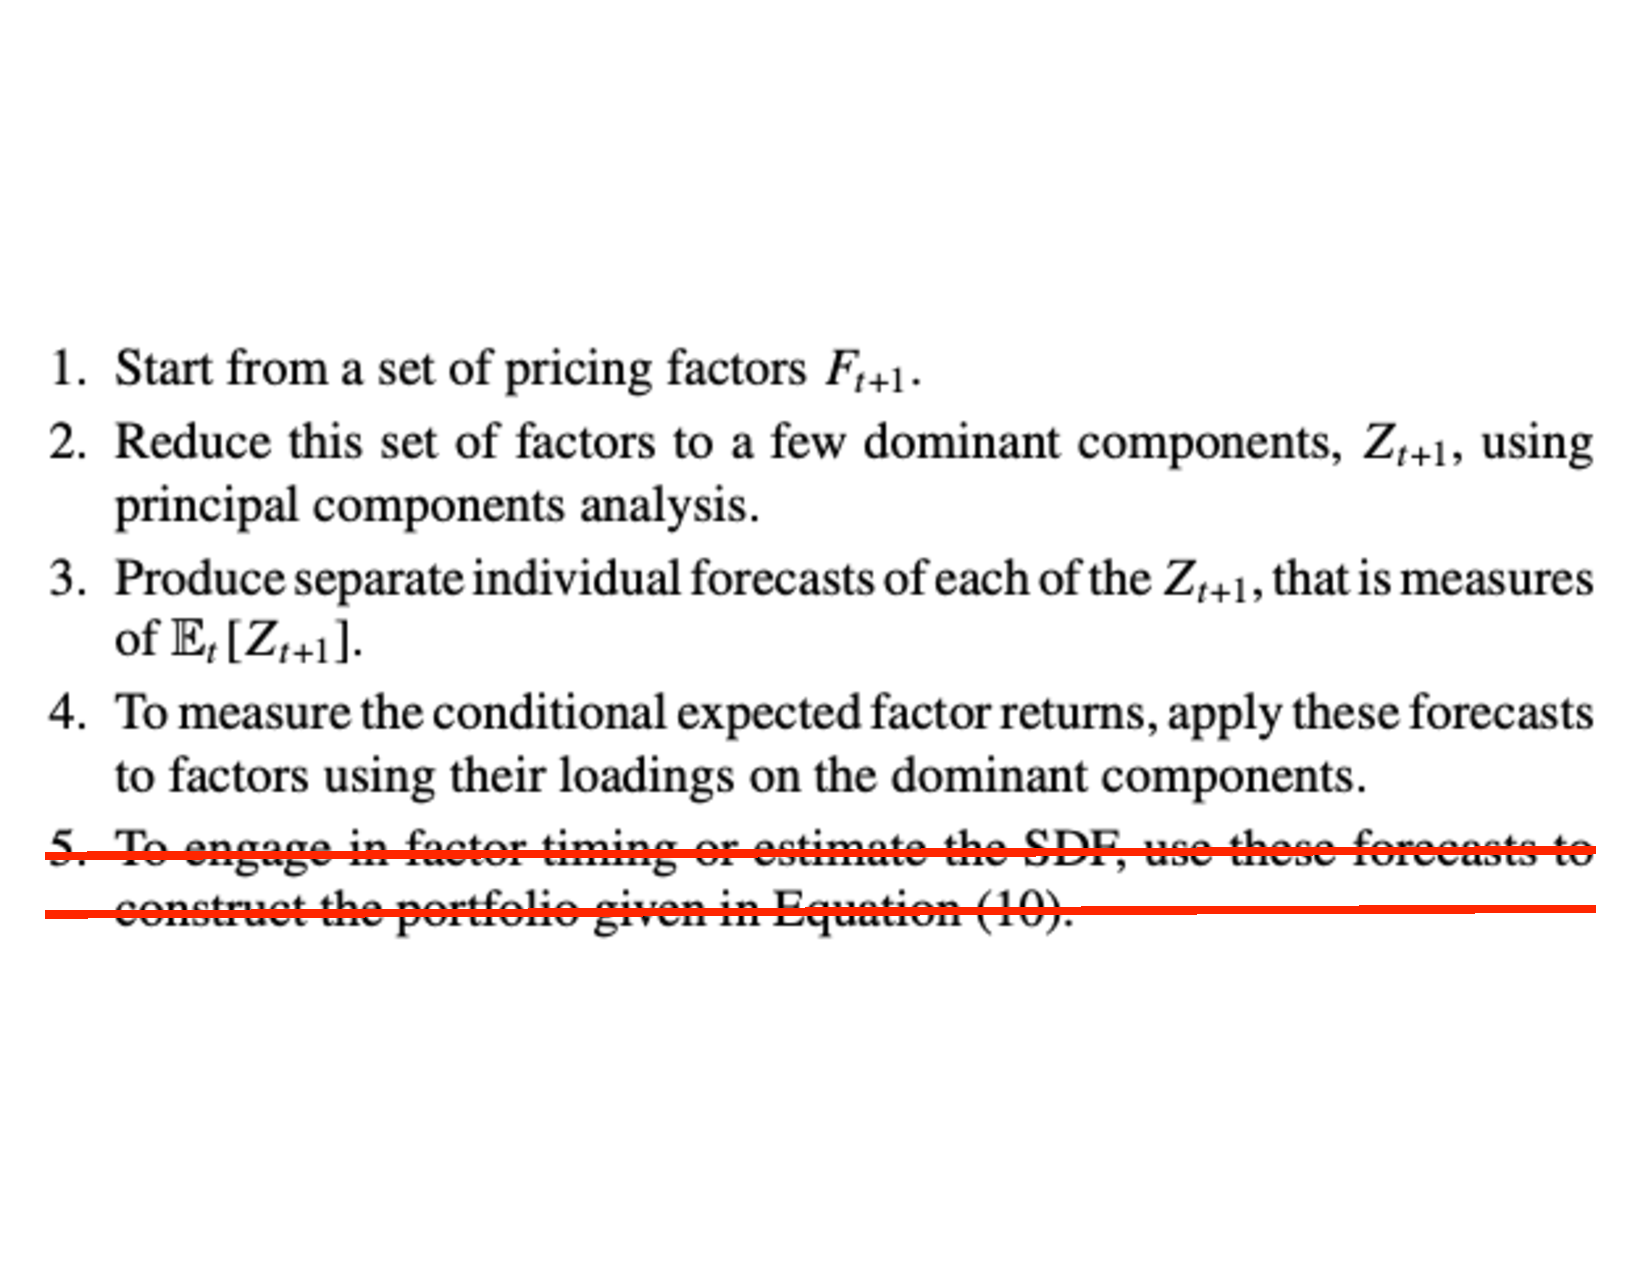
\includegraphics[width=300pt]{Steps_canceled.pdf}
	\end{figure}
\end{frame}

\begin{frame}{Methodology}
	\begin{itemize}
		\item Use \sout{fifty} fifty-five `anomaly' portfolios from Kozak et al. (2020)\footnote{\tiny Kozak, S., S. Nagel, and S. Santosh. 2020. Shrinking the cross-section. \textit{Journal of Financial Economics} 135:271–92.} that effectively capture market heterogeneity.
		\begin{itemize}
			\item These anomalies are the usual anomalies like Size, Value, ROA, SUE, etc.
		\end{itemize}
		\item Break them into deciles, create long-short portfolios for each anomaly (Decile 10 minus Decile 1).
		\begin{itemize}
			\item For each portfolio, they calculate the market-cap-weighted book-to-market ratio ($bm$) of the underlying stocks.
			\item By finding the difference in log book-to-market of Portfolio 10 minus that of Portfolio 1.
		\end{itemize}
		\item NOTE: This is a placeholder until we sort out data issues relating to `CMAs' (indexes).
	\end{itemize}
\end{frame}

\begin{frame}{Methodology}
	\begin{itemize}
		\item Market-adjust and rescale the data. 
		\begin{enumerate}
			\item Calculate regression $\beta$ for each anomaly. 
			\item Market-adjust returns and predictors by subtracting $\beta \times r_{mkt}$ for returns and $\beta \times bm_{mkt}$ for $bm$ ratios.
			\item Rescale to equalize the variance of market-adjiusted returns, and $bm$ ratios for each anomaly.
		\end{enumerate}
		\item So now they have \sout{50} 55 long-short portfolios.
	\end{itemize}
\end{frame}

\begin{frame}{Methodology}
	\begin{itemize}
		\item They conduct a PCA to reduce the \sout{50} 55 long-short portfolios to five PCs that explain roughly 60\% of the variance.
		\begin{figure}[!ht]
		\centering
			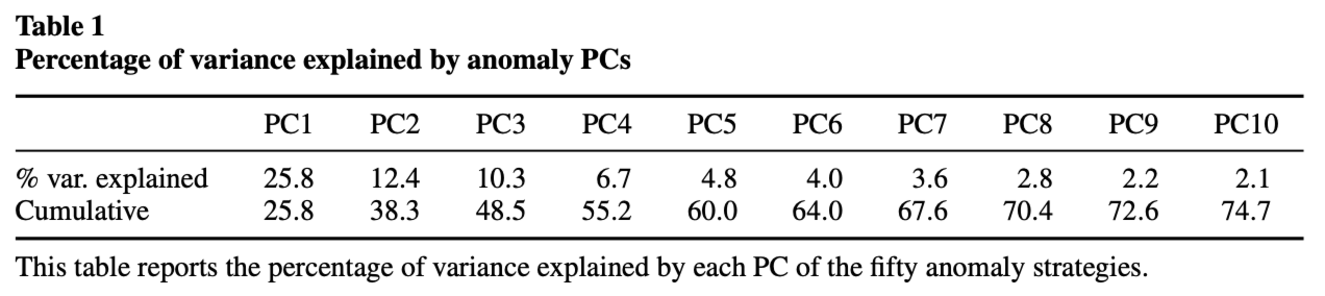
\includegraphics[width=250pt]{Table1.pdf}
		\end{figure}
		\item Why five? 
		\begin{enumerate}
			\item Campbell and Thompson (2007)\footnote{\tiny Campbell, J. Y., and S. B. Thompson. 2007. Predicting excess stock returns out of sample: Can anything beat the historical average? \textit{Review of Financial Studies} 21:1509–31.} show that the monthly $R^2$ when predicting the market is around 75bp.
			\item A loose upper-bound on the annual Sharpe is 1, or 8.3\% monthly. 
		\end{enumerate}
		\item If each included PC contributes equally to the $R^2$, the harmonic mean of their contribution to the total variance of returns must be $> \frac{0.75}{8.3} \approx 9\%$.
	\end{itemize}
\end{frame} 

\begin{frame}{Methodology}
	We extend the Haddad et al. study in the following way:
	\begin{enumerate}
		\item Asset class reduction using PCA/SVD.
		\item Regression analysis of principal components on factors (store coefficients).
		\item Calculate expected returns of factors.
		\item ToDo:
		\begin{enumerate}
			\item Calculate variance-covariance matrix of factors using regression coefficients, historical data, and residuals.
			\begin{itemize}
				\item Assume serial correlation.
			\end{itemize}
			\item Use asset-level factor loadings from G3 to get asset-level CMAs.
			\item Myriad data issues.
		\end{enumerate}
	\end{enumerate}
\end{frame}

\section{Background}

\begin{frame}{Literature}{Factor Models}
	\begin{itemize}
		\item The original one-factor model is the CAPM (Treynor (1961, 1962), Sharpe (1964), Lintner (1965) and Mossin (1966)).
		\item This was followed of course by Fama-French's three-factor (1993), and five-factor (2014) model.
		\item Between 1961 and the present, several hundred factors have been used to explain market inefficiency, market risk, and more.
		\begin{itemize}
			\item This led to the phenomenon commonly termed the `factor zoo', or the numerous factors used to explain stock market returns.
		\end{itemize}
	\end{itemize}
\end{frame}

\begin{frame}{Literature}{Factor Zoo}
	\begin{itemize}
		\item What is the `factor zoo'?
		\begin{itemize}
			\item First mentioned in Harvey, Liu, and Zhang (2016) following McLean and Pontiff (2015).
			\item Main issue is the proliferation of factors -- they test 316!
			\item They find that many of these factors are highly correlated.
		\end{itemize}
		\item So dimensionality reduction is highly recommended. This applies to our CMA problem as well.
		\begin{itemize}
			\item Envestnet, for example, has 55 asset classes. 
		\end{itemize}
	\end{itemize}
\end{frame}

\begin{frame}{Literature}{PCA}
	\begin{itemize}
		\item The use of PCA in asset pricing goes back to a series of papers by Connor and Korajczyk (1986, 1988, 1993).
		\item More recently, Kozak et al. (2020) have done work on dimensionality reduction of the cross-section of asset returns.
		\item Several other papers include: Kozak and Nagel (2023), Nadler and Sancetta (2023), and more\footnote{\tiny If you're interested, Fama and Stern (2016) have an interesting conversation on factor calculation using cross-sectional versus time series data.}.
%		\item More and more techniques have been used for this
%		\begin{itemize}
%			\item Related, but unrelated: 
%		\end{itemize}
	\end{itemize}
\end{frame}

%\begin{frame}{Literature}{Limitations}
%	\begin{itemize}
%		\item Most of the literature is used to explain risk premia 

\section{Data}

\begin{frame}{Data}
	\begin{itemize}
		\item We start with the anomaly dataset used in Haddad, Kozak, Santosh (2020) and Giglio, Kelly, Kozak (2020).
		\item Dataset consists of decile data along 55 equity anomalies.
		\begin{itemize}
			\item These consist of characteristics like size, value, momentum, reversal, etc.
		\end{itemize}
		\item Why this dataset? 
		\begin{itemize}
			\item It is easily accessible, and organized well.
			\item It serves as a good placeholder for CMA data.
			\item It is the same database used in Haddad et al. 
		\end{itemize}
	\end{itemize}
\end{frame}

\begin{frame}{Data}{Anomaly Dataset (Subset)}
	\begin{figure}[!ht]
		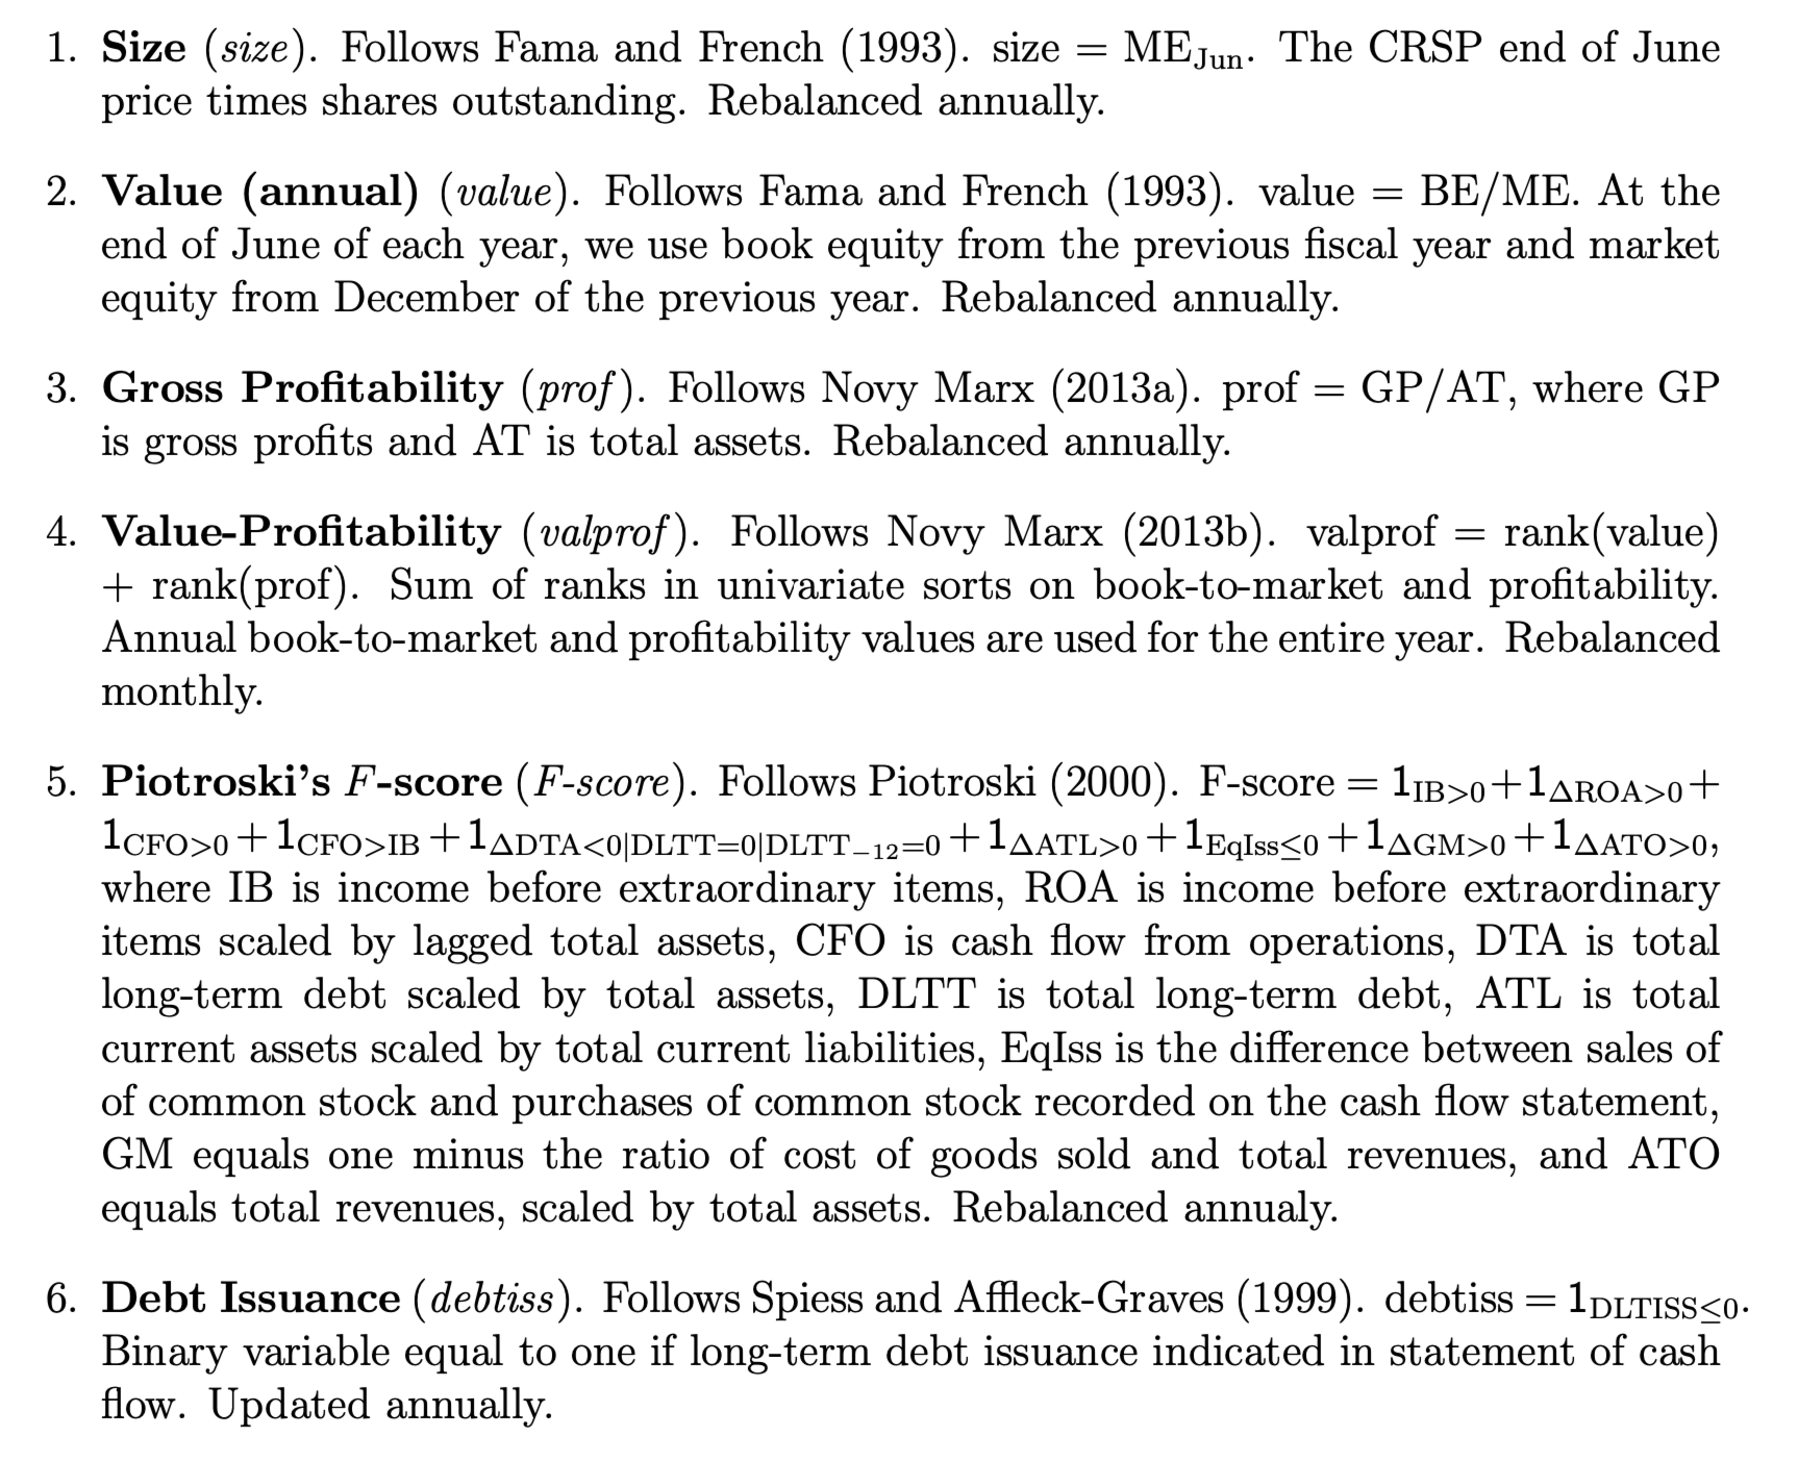
\includegraphics[width=200pt]{anomaly_definitions_subset.pdf}
		\caption{\footnotesize Start date: 07-01-2004. End date: 2019-12-01. Size: 186 x 54.}
	\end{figure}
\end{frame}

\begin{frame}{Data}{Factor Data}
	\begin{figure}[!ht]
		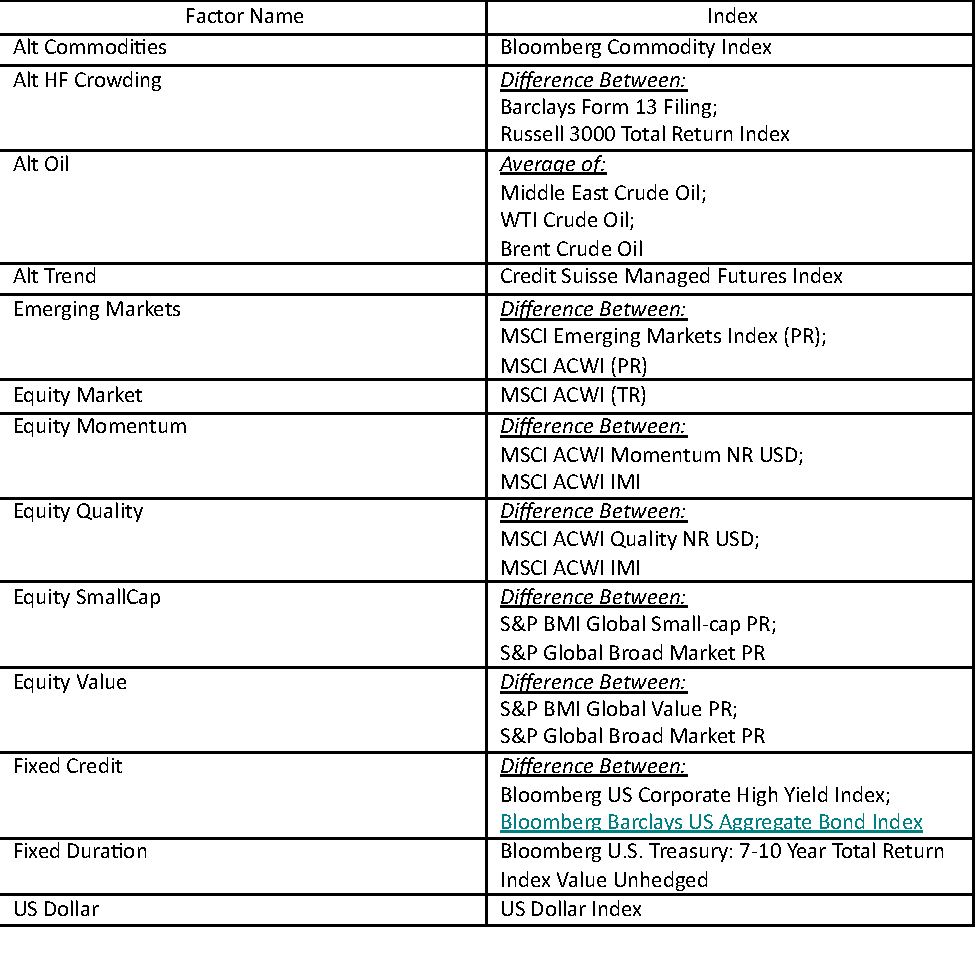
\includegraphics[width=175pt]{FactorDefinitions.pdf}
		\caption{\footnotesize Start date: 07-01-2004. End date: 2019-12-01. Size: 186 x 13.}
	\end{figure}
\end{frame}

\section{Results}

\begin{frame}{Results\footnote{\tiny Caveat: these results should be used for idea generation and for code plcaeholders; not taken literally.}}
	{\tiny Caveat: these results should be used for idea generation and for code plcaeholders; not taken literally.}
	\begin{itemize}
		\item Let's start with the dimensionality reduction for the anomalies dataset.
	\end{itemize}
	\begin{figure}[!ht]
		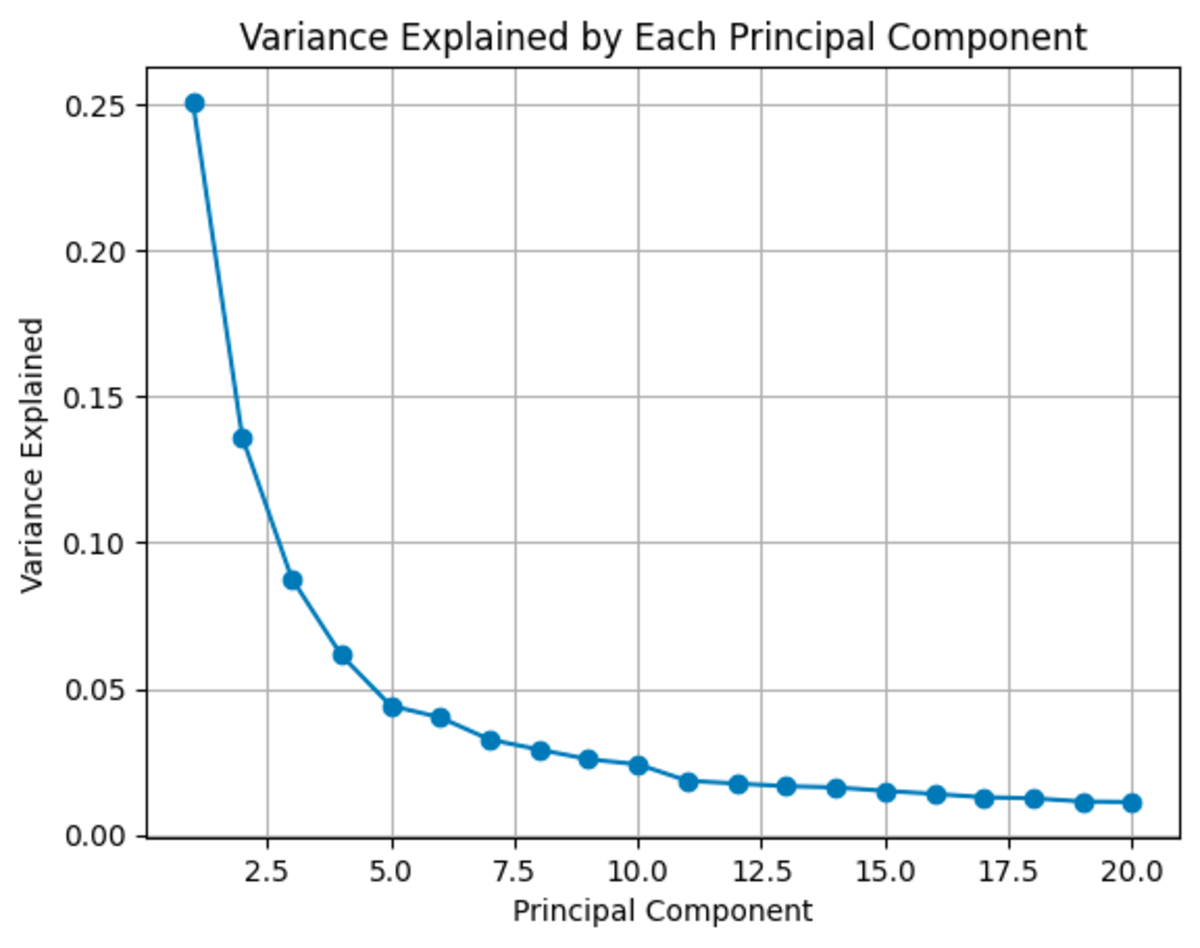
\includegraphics[width=175pt]{scree_plot.pdf}
		\caption{\footnotesize Scree plot}
	\end{figure}
\end{frame}	

\begin{frame}{Results\footnote{\tiny Caveat: these results should be used for idea generation and for code plcaeholders; not taken literally.}}
	\begin{figure}[!ht]
		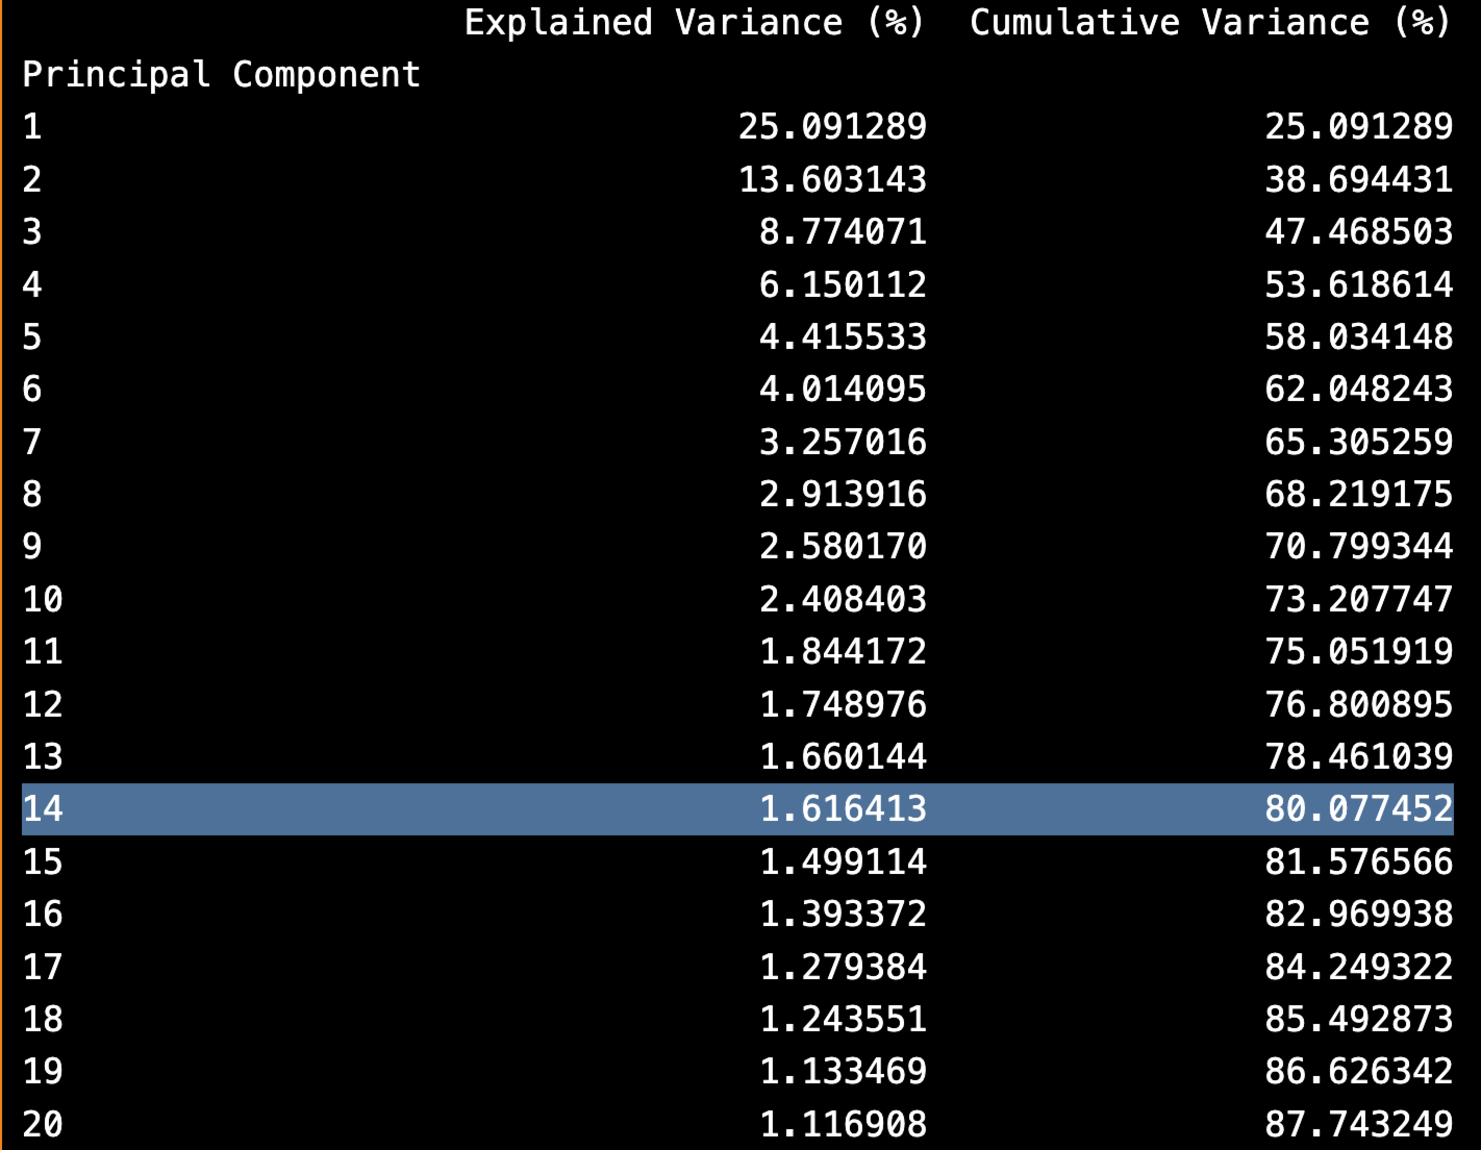
\includegraphics[width=200pt]{explained_variance.pdf}
	\end{figure}
	\begin{itemize}
		\item Roughly 80\% of the variance is explained by 14 principal components. 
	\end{itemize}
\end{frame}	

\begin{frame}{Results\footnote{\tiny Caveat: these results should be used for idea generation and for code plcaeholders; not taken literally.}}
	\begin{itemize}
		\item Running a OLS regression with HAC-robust standard errors, we get, for Alt Commodities:
	\end{itemize}
	\begin{figure}[!ht]
		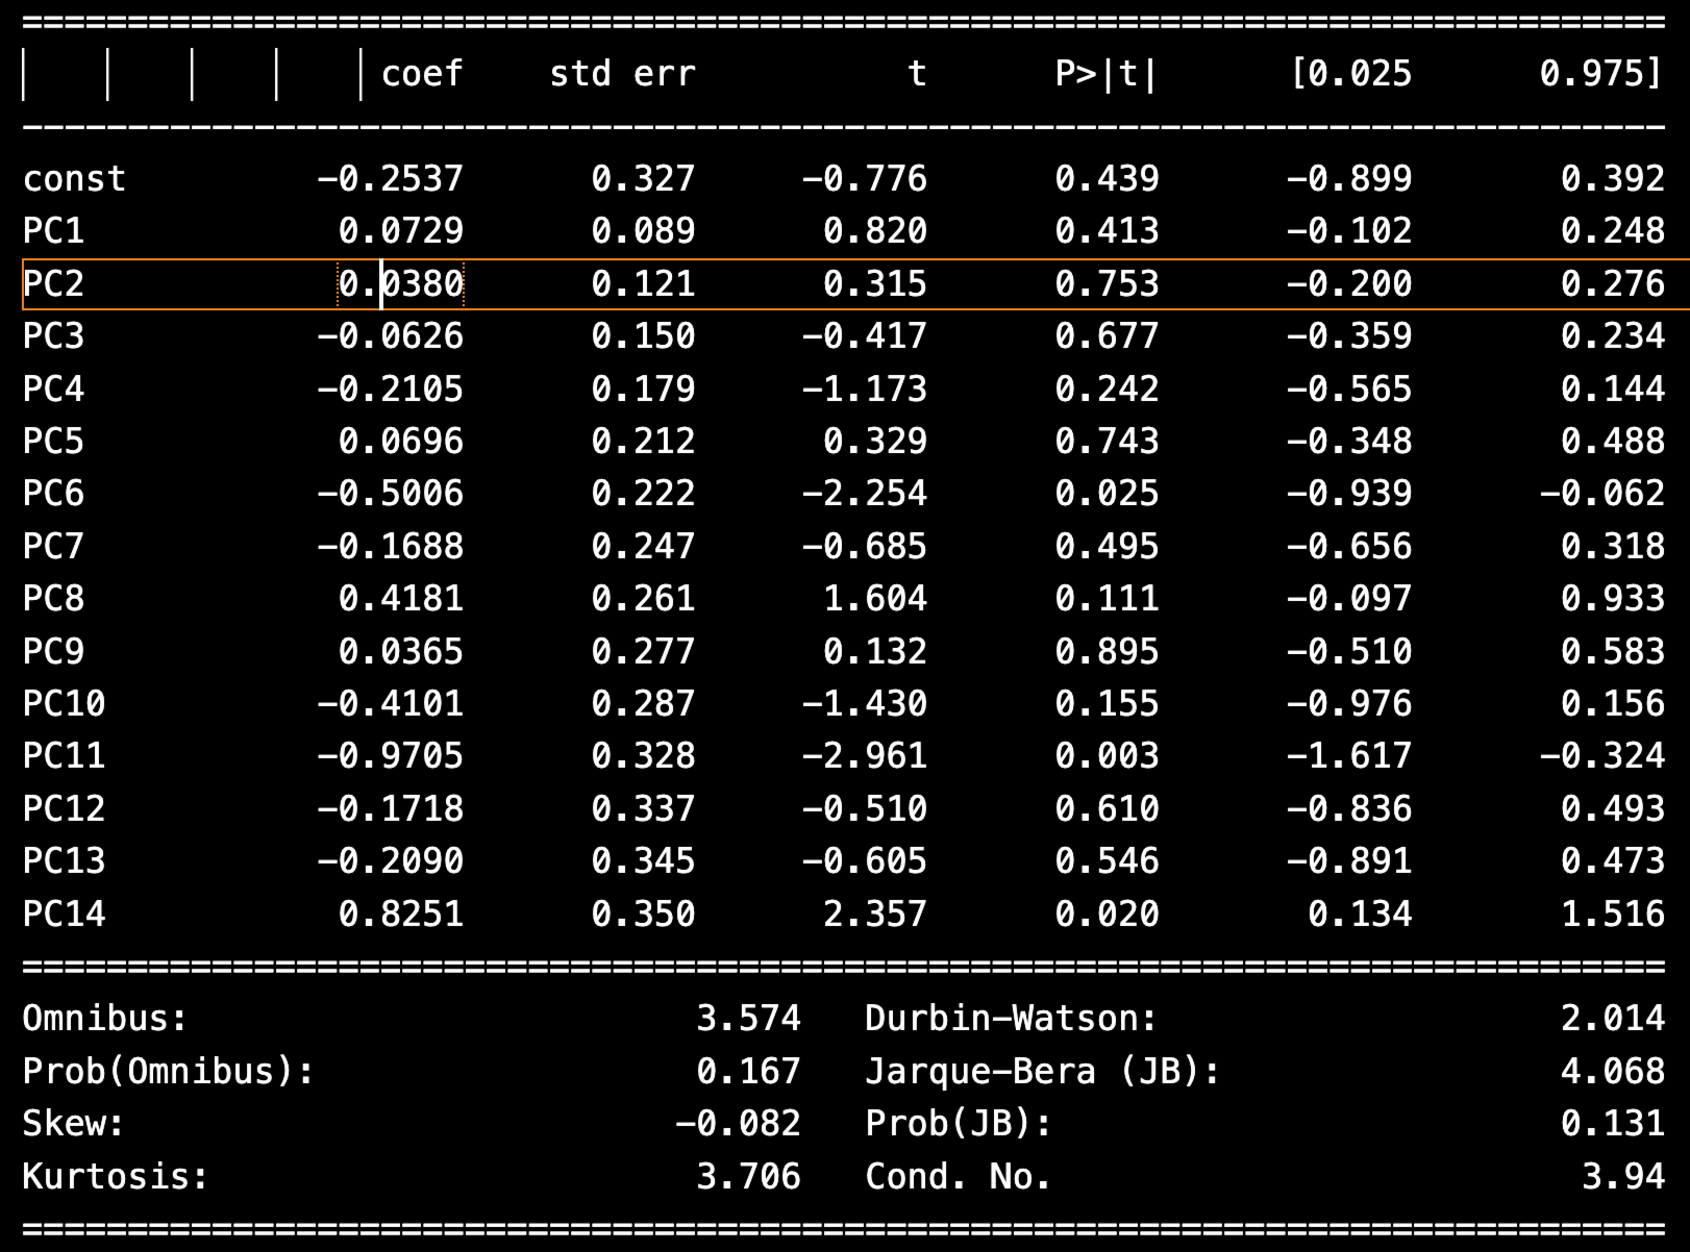
\includegraphics[width=200pt]{alt_commodities.pdf}
	\end{figure}
\end{frame}

\begin{frame}{Results\footnote{\tiny Caveat: these results should be used for idea generation and for code plcaeholders; not taken literally.}}
	\begin{itemize}
		\item Perhaps run a stepwise regression instead?
	\end{itemize}
	\begin{figure}[!ht]
		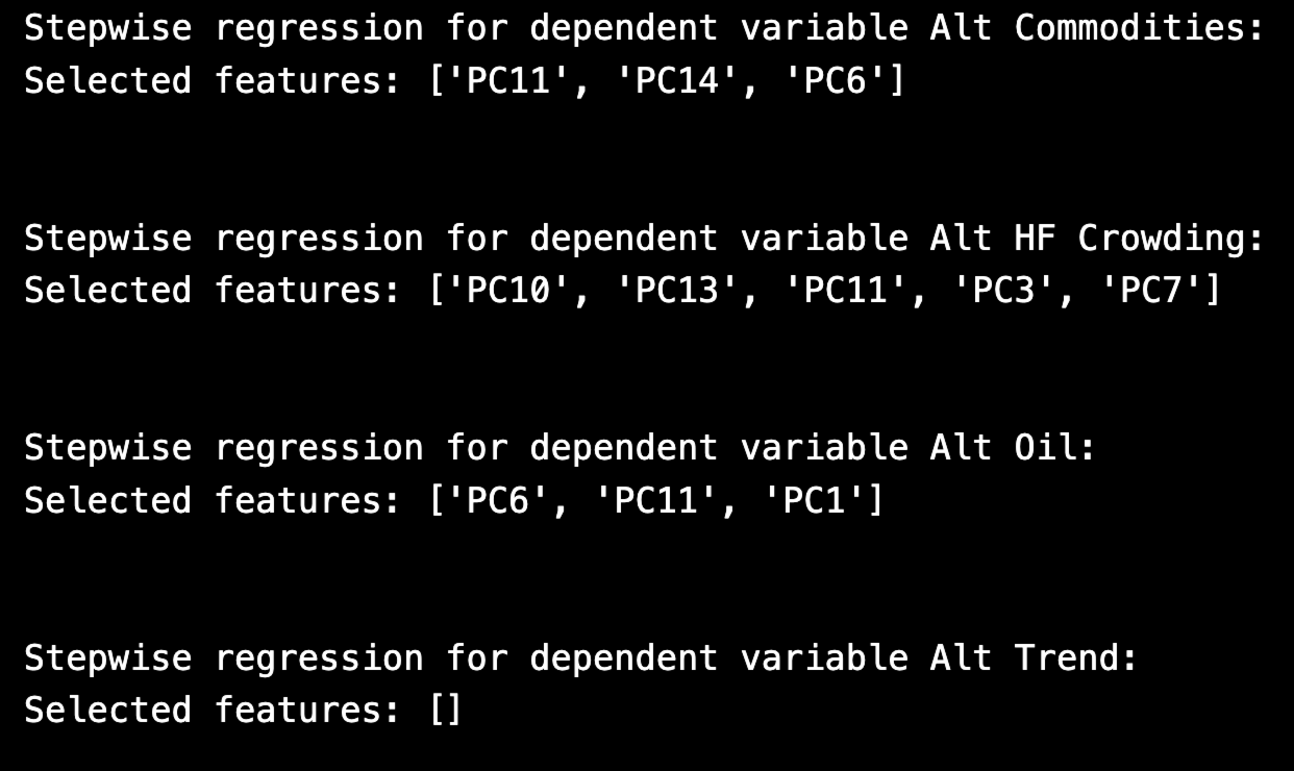
\includegraphics[width=200pt]{stepwise_results_subset.pdf}
	\end{figure}
\end{frame}


\begin{frame}{Issues}
	\begin{itemize}
		\item How do we use the CMA expected returns to `plug' into our regression results?
		\begin{itemize}
			\item Reconstructing the original matrix using reverse-SVD results in a high MSE\footnote{\tiny Thanks, Aniket, for your help here.}.
			\begin{itemize}
				\item Rabbit-hole: We can use Frobenius norm-minimization techniques for reconstruction.
			\end{itemize}
			\item Take the median of the respective PCs as substitutes for the historical expected returns? (Simplest solution, IMHO).
			\item Use the means of the original dataset and run another PCA with the same number of components?
		\end{itemize}
		\item Do we even want to follow this approach of using external CMAs to generate asset-level CMAs?
	\end{itemize}
\end{frame} 

\begin{frame}{Issues}
	\begin{itemize}
		\item How do we generate variance-covariance matrices using the PCA plus regression approach?
		\begin{itemize}
			\item We must account not only for the coefficient uncertainty but also the contribution to variance of each individual PC.
		\end{itemize}
	\end{itemize}
\end{frame}

\end{document}